\documentclass[notes,10pt, aspectratio=169]{beamer}


\usepackage{pgfpages}
% These slides also contain speaker notes. You can print just the slides,
% just the notes, or both, depending on the setting below. Comment out the want
% you want.
\setbeameroption{hide notes} % Only slide
%\setbeameroption{show only notes} % Only notes
% \setbeameroption{show notes on second screen=right} % Both

\usepackage{import}
% \usepackage{helvet} %? to change the font to Helvetica
% \usepackage[default]{lato}
% \usepackage{verbatim}

\usepackage{array}
% \usepackage{natbib}
% \bibliographystyle{plain}
\usepackage{apalike}
\bibliographystyle{apalike}
% \usepackage[natbib, maxcitenames=3, mincitenames=11, style=apa]{biblatex}

% \usepackage{fontspec} %! error

% \usefonttheme{professionalfonts} % using non standard fonts for beamer
% \usefonttheme{serif} % default family is serif

% \setmainfont{Liberation Serif}

% \setsansfont{Liberation Serif}


\usepackage{tikz}
\newcommand*\circled[4]{\tikz[baseline=(char.base)]{
 \node[shape=circle, fill=#2, draw=#3, text=#4, inner sep=2pt] (char) {#1};}}



\setbeamertemplate{note page}{\pagecolor{yellow!5}\insertnote}
\usetikzlibrary{positioning}
\usetikzlibrary{snakes}
\usetikzlibrary{calc}
\usetikzlibrary{arrows}
\usetikzlibrary{decorations.markings}
\usetikzlibrary{shapes.misc}
\usetikzlibrary{matrix,shapes,arrows,fit,tikzmark}
\usepackage{amsmath}
\usepackage{mathpazo}
\usepackage{hyperref}
\usepackage{lipsum}
\usepackage{multimedia}
\usepackage{graphicx}
\usepackage{multirow}
\usepackage{graphicx}
\usepackage{dcolumn}
\usepackage{bbm}
\usepackage{cancel}
\newcolumntype{d}[0]{D{.}{.}{5}}
\usepackage{subcaption}
\usepackage{changepage}
\usepackage{appendixnumberbeamer}
\newcommand{\beginbackup}{
 \newcounter{framenumbervorappendix}
 \setcounter{framenumbervorappendix}{\value{framenumber}}
 \setbeamertemplate{footline}
 {
 \leavevmode%
 \hline
 box{%
 \begin{beamercolorbox}[wd=\paperwidth,ht=2.25ex,dp=1ex,right]{footlinecolor}%
% \insertframenumber \hspace*{2ex} 
 \end{beamercolorbox}}%
 \vskip0pt%
 }
 }
\newcommand{\backupend}{
 \addtocounter{framenumbervorappendix}{-\value{framenumber}}
 \addtocounter{framenumber}{\value{framenumbervorappendix}} 
}


\usepackage{graphicx}
\usepackage[space]{grffile}
\usepackage{booktabs}

% These are my colors -- there are many like them, but these are mine.
\definecolor{blue}{RGB}{70,160,205}
\definecolor{red}{RGB}{213,94,0}
\definecolor{yellow}{RGB}{240,228,66}
\definecolor{green}{RGB}{0,158,115}

% % Enviroments
% \newtheorem{defin}{Definition.}
% \newtheorem{teo}{Theorem. }
% \newtheorem{lema}{Lemma. }
% \newtheorem{coro}{C
% \begin{frame}{Modeling Choice}orolary. }
% \newtheorem{prop}{Proposition. }
% \theoremstyle{definition}
% \newtheorem{examp}{Example. }
% % \numberwithin{problem}{subsection} 

\hypersetup{
 colorlinks=false,
 linkbordercolor = {white},
 linkcolor = {blue} 
}

\newcommand\Fontvi{\fontsize{8.5}{7.2}\selectfont}

\newcommand\Fontx{\fontsize{10}{7.2}\selectfont}
%% I use a beige off-white for my background
\definecolor{MyBackground}{RGB}{255,253,218}

%% Uncomment this if you want to change the background color to something else
%\setbeamercolor{background canvas}{bg=MyBackground}

%% Change the bg color to adjust your transition slide background color!
\newenvironment{transitionframe}{
 \setbeamercolor{background canvas}{bg=white}
 \begin{frame}}{
 \end{frame}
}

\setbeamercolor{frametitle}{fg=blue}
\setbeamercolor{title}{fg=black}
\setbeamertemplate{footline}[frame number]
\setbeamertemplate{navigation symbols}{} 
\setbeamertemplate{itemize items}{-}
% \setbeamertemplate{itemize items}[circle]   
% \setbeamertemplate{itemize subitem}[triangle]
% \setbeamertemplate{itemize subsubitem}[circle]
% \setbeamertemplate{enumerate items}[default]
% \setbeamertemplate{section in toc}[circle]
% \setbeamertemplate{subsection in toc}[triangle]
% \setbeamertemplate{subsubsection in toc}[square]


\setbeamercolor{itemize item}{fg=blue}
\setbeamercolor{itemize subitem}{fg=blue}
\setbeamercolor{itemize subsubitem}{fg=blue}
\setbeamercolor{enumerate item}{fg=blue}
\setbeamercolor{enumerate subitem}{fg=blue}
\setbeamercolor{enumerate subsubitem}{fg=blue}
\setbeamercolor{button}{bg=MyBackground,fg=blue,}
\setbeamercolor{theotem}{fg=blue} 

% If you like road maps, rather than having clutter at the top, have a roadmap show up at the end of each section 
% (and after your introduction)
% Uncomment this is if you want the roadmap!
%\AtBeginSection[]
%{
% \begin{frame}
% \frametitle{Roadmap of Talk}
% \tableofcontents[currentsection]
% \end{frame}
%}

%  buttons transparent:
% \setbeamertemplate{button}{\tikz
%  \node[
%  inner xsep=10pt,
%  draw=structure!80,
%  fill=structure!50,
%  rounded corners=4pt]  {\insertbuttontext};}

\setbeamercolor{section in toc}{fg=blue}
\setbeamercolor{subsection in toc}{fg=red}
\setbeamersize{text margin left=1em,text margin right=1em} 

\newenvironment{wideitemize}{\itemize\addtolength{\itemsep}{10pt}}{\enditemize}

\usepackage{environ}
\NewEnviron{videoframe}[1]{
 \begin{frame}
 \vspace{-8pt}
 \begin{columns}[onlytextwidth, T] % align columns
 \begin{column}{.58\textwidth}
 \begin{minipage}[t][\textheight][t]
 {\dimexpr\textwidth}
 \vspace{8pt}
 \hspace{4pt} {\Large \sc \textcolor{blue}{#1}}
 \vspace{8pt}
 
 \BODY
 \end{minipage}
 \end{column}%
 \hfill%
 \begin{colußmn}{.42\textwidth}
 \colorbox{green!20}{\begin{minipage}[t][1.2\textheight][t]
 {\dimexpr\textwidth}
 Face goes here
 \end{minipage}}
 \end{column}%
 \end{columns}
 \end{frame}
}
% * Changing Font



% Unraveling Deposit Dynamics: Local Bank Competition and Segmented Deposit Markets

\title[]{\textcolor{blue}{The Digital Banking Revolution: \\
Effects on Competition and Stability}} %, Rate Dispersion and Profits in 

\subtitle{\textcolor{blue}{Naz Koont (2024)}\footnote{
 Stanford University, Graduate School of Business
}}
\author{Presenter: Giselle Labrador-Badia}
% university
\institute{University of Wisconsin-Madison}
%\centering
\date{\today}


\begin{document}
%%% TIKZ STUFF
\tikzset{ 
 every picture/.style={remember picture,baseline},
 every node/.style={anchor=base,align=center,outer sep=1.5pt},
 every path/.style={thick},
 }
\newcommand\marktopleft[1]{%
 \tikz[overlay,remember picture] 
 \node (marker-#1-a) at (-.3em,.3em) {};%
}
\newcommand\markbottomright[2]{%
 \tikz[overlay,remember picture] 
 \node (marker-#1-b) at (0em,0em) {};%
}
\tikzstyle{every picture}+=[remember picture] 
\tikzstyle{mybox} =[draw=black, very thick, rectangle, inner sep=10pt, inner ysep=20pt]
\tikzstyle{fancytitle} =[draw=black,fill=red, text=white]
%%%% END TIKZ STUFF

% % Title Slide
\begin{frame}[noframenumbering]
 \maketitle
\end{frame}



\begin{frame}{Introduction}

    \vspace{0.2cm}

    \begin{wideitemize}
        % \item Deregulation story: short until Riegle Act
        \item %\textcolor{blue}{Background:}
 Digital banking platforms have become widespread as an alternative to traditional physical branches.
        \item Effects on competition are unclear: 
        
        \vspace{0.2cm}
        \begin{wideitemize}
            \item size distributions of banks (scale economies, lower investment costs),
            \item banking products (loans, deposits).

        \end{wideitemize}
        \item Competition $\rightarrow$ stability.
        \pause
        \item \textcolor{blue}{How does the digital revolution affect competition and stability?} 

        % \item \textcolor{blue}{Preview of results}:
            \vspace{0.2cm}
            \begin{wideitemize}
                \vspace{0.2cm}
                \item  $\uparrow$ competition, $\downarrow$ stability.

            \end{wideitemize}

        % \item 

    \end{wideitemize}
    % \item Banks compete for deposits

\end{frame}

\begin{frame}{Introduction}

    \begin{wideitemize}
      
        \item \textcolor{blue}{Preview of results}:

    % \item \textcolor{blue}{Preview of results}:
        \vspace{0.2cm}
        \begin{wideitemize}
            \vspace{0.2cm}
            \item  $\uparrow$ competition, $\downarrow$ stability.
            \item After digitalization:
            \vspace{0.2cm}
            \begin{itemize} 
                \item banks operate in more markets, and mid-size banks grow faster.
            \item More uninsured deposits in balance sheets, and more loans to high-income borrowers.
            \end{itemize}
            \item Structural model of the U.S. banking industry to compare counterfactual without digitalization.

            % \item Provide a theory that rationalizes the observed patterns (framework Oberfield et al. (2024)).
            \begin{itemize}
                \vspace{0.2cm}
                \item $\uparrow$ competition, $\downarrow$ stability.
                \item $\uparrow$ consumer surplus and banks profits. 

            \end{itemize}

        \end{wideitemize}


    \end{wideitemize}
\end{frame}

\begin{frame}{Introduction}

    \begin{wideitemize}
        
        \item \textcolor{blue}{Contribution:} 
                \vspace{0.2cm}
        \begin{wideitemize}
            \item How digital platforms alter competition in banking. \footnote{Dreschsler et al. (2017), Honka et al. (2014), Hatfield and Wallen (2022), Vives and Ye (2022), Jiant et al. (2020)}
    
            \item Effects on banks' screening and monitoring abilities by finding greater per-unit loan losses and more loans to high-income borrowers.
            \footnote{Fishman et al. (2017), Stein (2022), and Gornall et al. (2023), Di Maggio and Yao (2021), Liberti and Petersen (2019)}
            
            \item Effect on digital platforms on banks' funding composition and stability. \footnote{Diamond and Dybvig (1983), Egan et al. (2019), Jiang et al. (2023), Drechler et al. (2023), Benmelech et al. (2023).}
        
            \item Banks technology adoption by endogenizing digital platform adoption. \footnote{Vives (2019), Jiang et al. (2022), Haendler (2022).}
            

        \end{wideitemize}
        % \item Banks compete for deposits
    \end{wideitemize}
    
\end{frame}
    
    
    
\begin{frame}{Data}
    
    \begin{wideitemize}
        \item Digital platform adoption
        \vspace{0.2cm}
        \begin{itemize}
            \item Construction of data set for the universe of U.S. banks. 
            \item Release date of each bank's mobile application on Apple and Android App Stores, banking application's features, and its rating. 
            \item[$\rightarrow$] Dummy variable of whether banks have a mobile application at the start of each year.
   
        \end{itemize} 

        \item Other data sources: 
        \begin{itemize} 
            \vspace{0.2cm}
   
            \item Call Reports, SDI, RateWatch,
            \item mortgage: HMDA, small business loans: CRA, FinTech mortgage,
            \item FCC census block-level data on broadband availability.
        \end{itemize}
        % \item County-level data on population and income from the Census and BEA.
        \item Sample: unbalanced annual panel of U.S. commercial banks from 2010 to 2019.\footnote{Banks with more than 0.001\% market share and at least 5 branches.}
    \end{wideitemize}
    
\end{frame}
    


   % frame with figure

\begin{frame}{Digital Banking Platform Adoption and Market Concentration}

    \begin{itemize}
        \item Digital platforms rise coincides with attenuation of market concentration.
        \item Suggest that digital platforms may have increased competition.
    \end{itemize}

    \begin{figure}
        \centering
        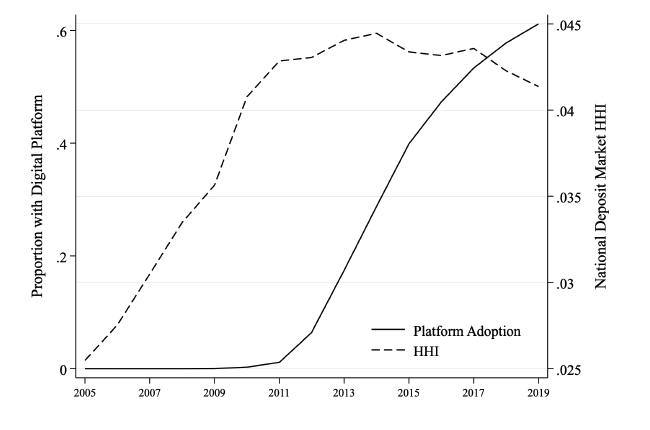
\includegraphics[width=0.64\textwidth]{imgs/fig1.png}
    \end{figure}

\end{frame}

\begin{frame}{Institutional Background Main Features}

    \begin{wideitemize}

        \item Dramatic increase in platform adoption after 2010.

        \item By 2019, 60\% of banks will have a mobile banking application.
        
        \item Top mobile common features are access to account balances, transaction history, transfer money, find branches and ATMs, and mobile check deposits and loans. 

        \item Most banks (60\%) report getting services from third-party providers (FIS, Fiserv, Jack Henry).
        
        \item Digital platform quality varies across the bank size distribution (see next slide).


    \end{wideitemize}

\end{frame}


\begin{frame}{Banks' digital platform quality and branch ratings}

    \begin{itemize}
        \item Larger banks have more mobile features and better app ratings. 
        \item Smaller banks have better branch ratings.\footnote{Panel B includes county fixed effects.}
    \end{itemize}
    \begin{figure}
        \centering
        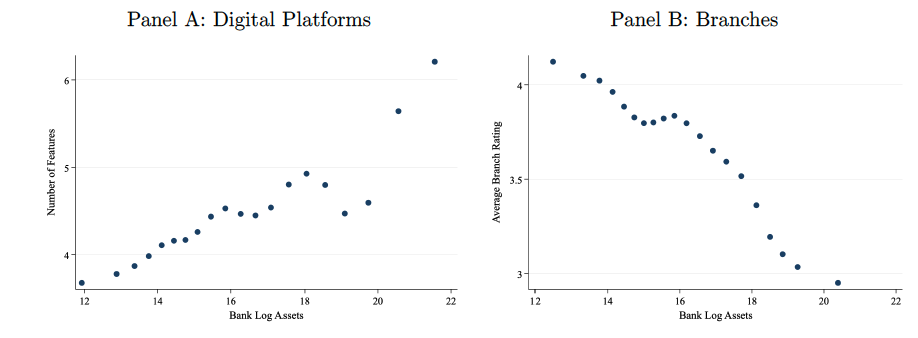
\includegraphics[width=0.92\textwidth]{imgs/fig3.png}
        %\caption*{Caption}
        \label{fig:my_label}
    \end{figure}
    
    \end{frame}


% ********************************************************************************************************************
\begin{frame}[noframenumbering]

    % {Evidence of Sorting}   
    \huge \centering \textcolor{blue}{Empirical Strategy and Reduced Form Evidence}
\end{frame}


\begin{frame}{Instrument construction and identification}

    \begin{itemize}
        \item Digital adoption is endogenous (omitted variable bias)
        \item Use banks' exposure to technology that facilitates digitalization.
        \item Use quasirandom availability of AT\&T's coverage relative to other carriers.

    \end{itemize}
    
    \begin{figure}
        \centering
        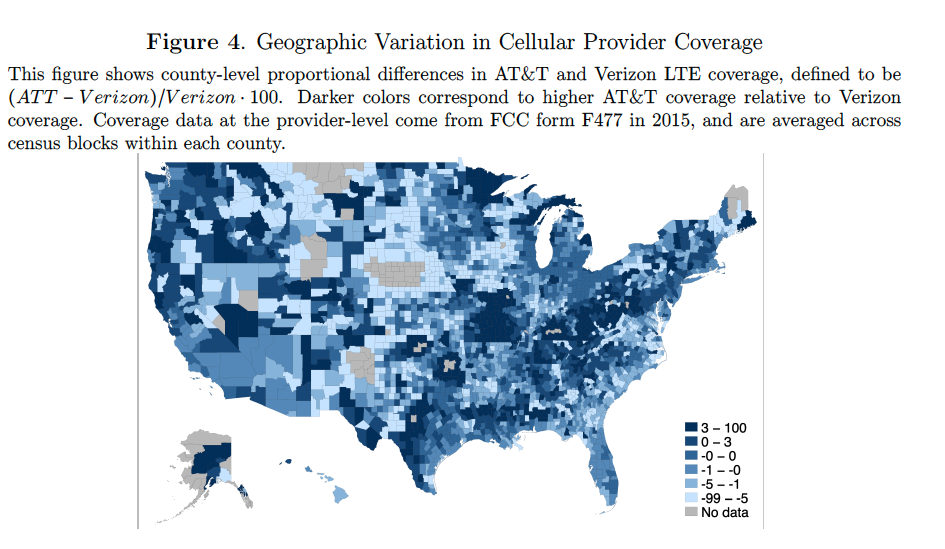
\includegraphics[width=0.76\textwidth]{imgs/fig4.png}
        % \caption*{ The use of wholesale funds across the bank size distribution in 1984.}
        \label{fig:my_label}
    \end{figure}
    
\end{frame}

\begin{frame}{Instrument construction}


    \begin{wideitemize}
    \item The instrument for bank adoption of mobile services is: 

    $$
    \begin{aligned}
 Z_b & \equiv \sum_c \text { Shares }_{b, c} \cdot \text { Shocks }_c \\
        \text { Shocks }_c & \equiv \text { AT\&T }_c \\
        \text { Shares }_{b, c} & \equiv \frac{\text { Deposit Share }_{b, c} \cdot \text { Population }_c}{\sum_c \text { Deposit Share }_{b, c} \cdot \text {Population }_c}
        \end{aligned}
    $$

 Where $Z_b$ is a shift-share instrument for technology adoption and Shocks $_c$ is the AT\&T coverage in county $c$ (2015), deposits and population are measured in 2009.

    \pause
    \item Main regression specification is
    $$
    \begin{aligned}
        \text { Digital }_{b, t} & =\delta_1 Z_b+\delta_2 \text { Coverage }_b+\delta_3 X_{b, t}+\eta_{b, t} \\
        \mathrm{Y}_{b, t} & =\beta_1{\widehat{\text { Digital }_{b, t}}}{+\beta_2 \text { Coverage }_b+\beta_3 X_{b, t}+\varepsilon_{b, t}}
        \end{aligned}
    $$
 Coverage $_b$ is similar to $Z_b$ but with AT\&T and Verizon.

    \end{wideitemize}

\end{frame}


    
\begin{frame}{ATT Coverage as instrument}

% create two cols 


\begin{columns}[T]
    
    \begin{column}{0.5\textwidth}
    
    \begin{figure}
        \centering
        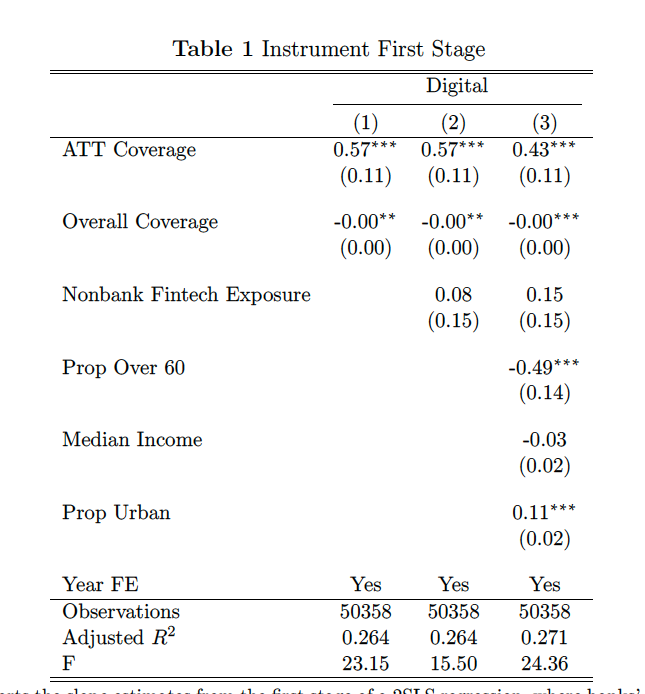
\includegraphics[width=0.95\textwidth]{imgs/tab1.png}
        % \caption*{ Standard errors  
        % are two-way clustered at the state and bank level.}
        % \label{fig:my_label}
    \end{figure}

\end{column}
\begin{column}{0.5\textwidth}
    

    % \begin{wideitemize}
        % \item \textcolor{blue}{Table 1:} 
        \begin{wideitemize}
            \item Bank-year level observations from 2010 to 2019, year FE. 
            \item Standard errors are clustered at the bank level. 
            \item Validity of the instrument:
                \begin{wideitemize}
            \item Relevance: increase in digital adoption with AT\&T coverage.
            \item Exclusion restriction: shift-share instruments if shares are exogenous. 
            \item Variation in AT\&T coverage might be as good as random.
            \item Banks' characteristics are not significantly correlated with instruments. 
        \end{wideitemize}
    \end{wideitemize}
\end{column}
\end{columns}


\end{frame}

\begin{frame}{Evidence of spatial sorting}

    % \begin{wideitemize}
    
        \begin{wideitemize}
            %How did this expansion affect spatial sorting patterns? 
            \item Local banking markets increase avg. No. of banks that are originating small business loans and mortgages.
            \item Expansion is not accompanied by a proportional increase in bank branch presence.
    \end{wideitemize}
    
    \begin{figure}
    \centering
    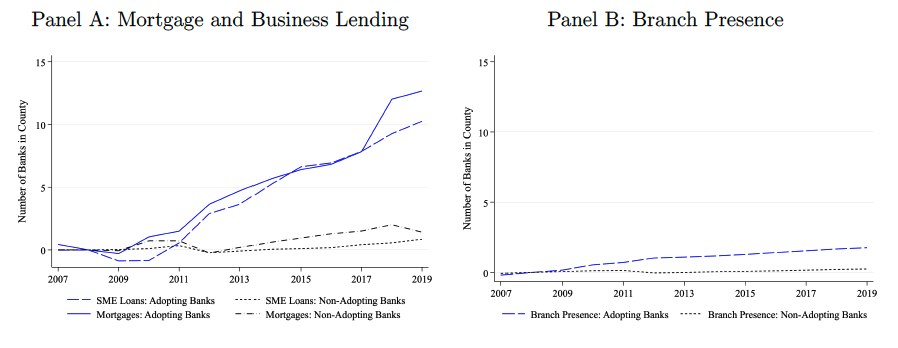
\includegraphics[width=0.99\textwidth]{imgs/fig5.png}
    %\caption*{Caption}
    \label{fig:my_label}
    \end{figure}
    
    \end{frame}
    
    

\begin{frame}{Bank Geographic expansion and digitalization}
% the sample to banks that are active in two or more counties to avoid headquarters location biases. 

\begin{wideitemize}
\item Banks that adopt digital platforms increase the no. of counties in which they originate by 86\%.
\end{wideitemize}
\begin{figure}
\centering
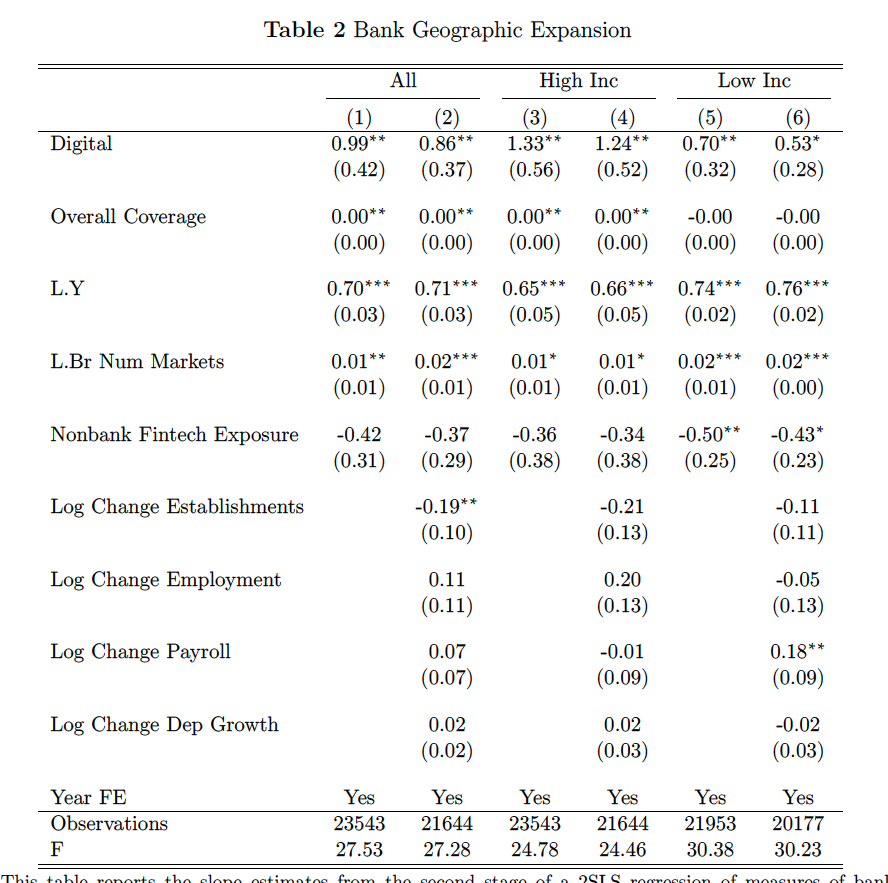
\includegraphics[width=0.8\textwidth]{imgs/tab2.png}
\caption*{Changes in relative and absolute sorting patterns between 1981 and 2006 for
four bank-size bins.\\ (a) Sorting interaction coefficients. (b) Distance coefficients.}
% (b) Distance coefficients.}
\label{fig:my_label}
\end{figure}

% \begin{itemize}

% \end{itemize}



\end{frame}


\begin{frame}{Bank branches' response to digitalization}

    \begin{itemize}
        \item Banks close branches after adopting digital platforms.
        \item Expand service provision. \
    \end{itemize}
\begin{figure}
    \centering
    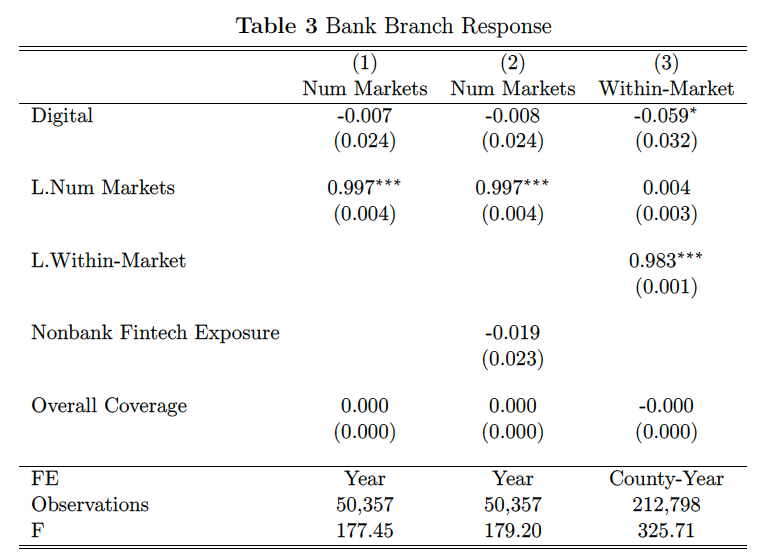
\includegraphics[width=0.65\textwidth]{imgs/tab3.png}
\end{figure}

\end{frame}


\begin{frame}{Banks balance sheet growth}
    \begin{wideitemize}
        \item U-shaped across bank size, mid-size banks grew more.
        \item Deposit growth of mid-size banks is elevated.
    \end{wideitemize}

    \begin{figure}
    \centering
    \begin{minipage}{0.9\textwidth}
 {\footnotesize
 Controls include establishments, employment, payroll, deposit, loan growth, and year fixed effects.}
        \end{minipage}
    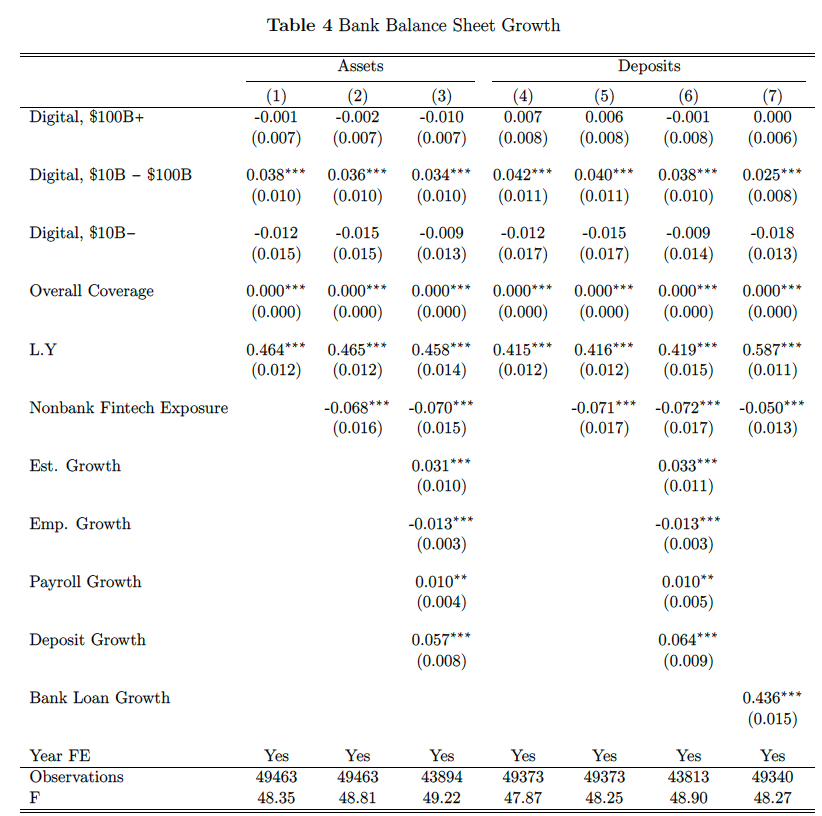
\includegraphics[width=0.85\textwidth]{imgs/tab4.png}
    \end{figure}
\end{frame}

\begin{frame}{Digital banking facilitates uninsured deposits}

\begin{itemize}
\item Growth in deposits among adopters is disproportionately in uninsured deposits.
\item Decrease of insured deposit for large and medium banks.
\end{itemize}


\begin{figure}
\centering
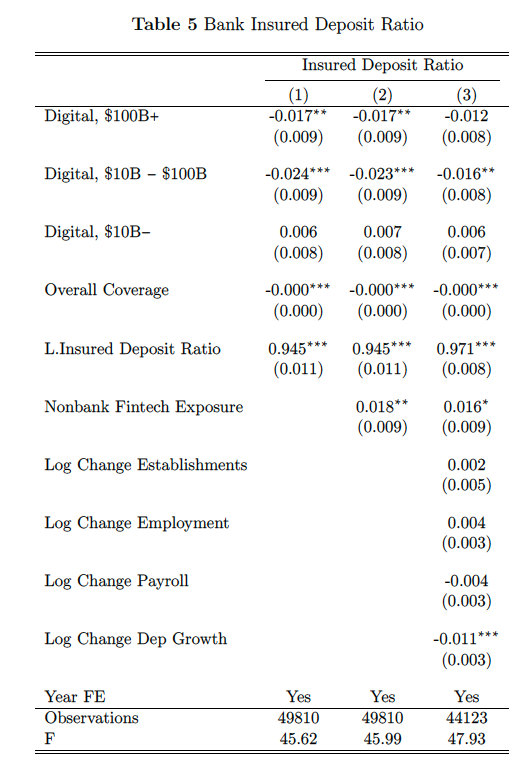
\includegraphics[width=0.5\textwidth]{imgs/tab5.png}
% \caption*{Sorting coefficients $\beta_t$ between 1981 and 2006.}
% \label{fig:my_label}
\end{figure}

\end{frame}



\begin{frame}{Corporate deposits are flowing to banks with digital platforms}
    % \begin{itemize}
    %     % \item conclusions of table here
    % \end{itemize}

    \begin{figure}
    \centering
    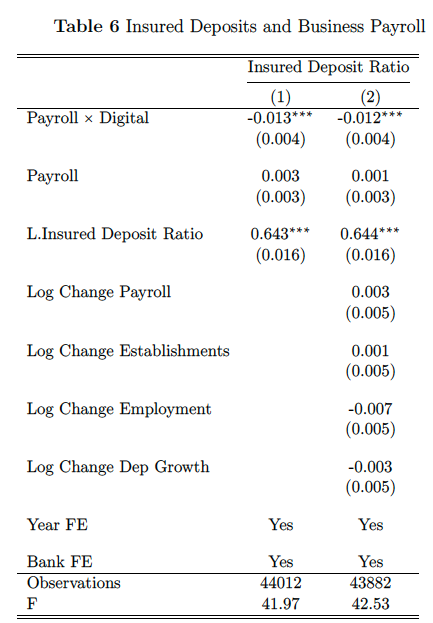
\includegraphics[width=0.4\textwidth]{imgs/tab6.png}
    %\caption*{Caption}
    % \label{fig:my_label}
    % \caption*{Standard errors are two-way clustered at the state and bank level.}
    \end{figure}

\end{frame}

\begin{frame}{Bank Low Income Mortgages in New Counties}

\begin{itemize}
\item Bank expansion into new counties driven by high-income borrowers.
\item Adopting banks reduce low-income mortgage origination by 27\%, volume by 38\%.
\end{itemize}
    \begin{figure}
        \centering
        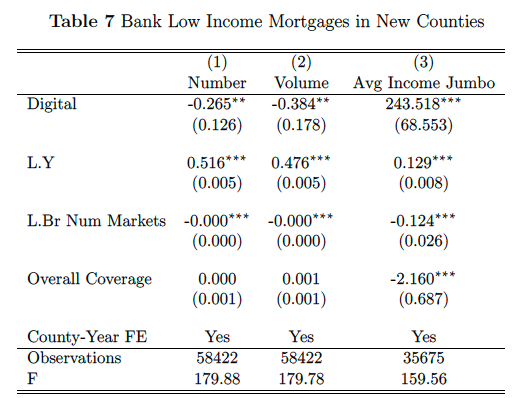
\includegraphics[width=0.5\textwidth]{imgs/tab7.png}
        %\caption*{Caption}
        % \label{fig:my_label}
    \end{figure}
    
\end{frame}

\begin{frame}{Loan Activity in New Counties}

    \begin{itemize}
        \item Increase overall mortgage applications, fewer from low-income borrowers.
        \item Around 76\% more rejections for low-income borrowers.
    \end{itemize}

    \begin{figure}
        \centering
        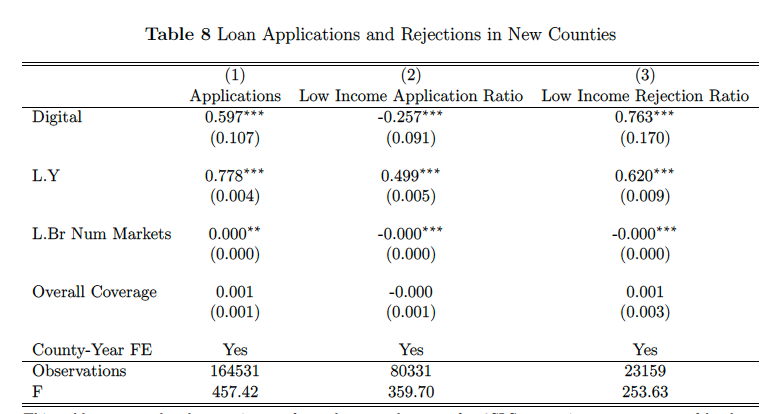
\includegraphics[width=0.875\textwidth]{imgs/tab8.png}
    \end{figure}
    
\end{frame}



% * Possible summary slide with evidence
% \begin{frame}{Connecting mismatch sorting to the level of wholesale funding}\label{mismatch_sorting}

% \vspace{0.1cm}

% \textcolor{blue}{Mismatch sorting:} Banks choose locations based on the match of the location's characteristics to the funding needs.
% %! Summary of the results
% \begin{wideitemize}
%     \item Denser locations are less deposit intensive \hyperlink{mismatch_sorting1}{\beamerbutton{Regression}}
    
%     \item Banks that were headquartered in counties with more loan opportunities used more wholesale funding in 1984. 
%     \hyperlink{mismatch_sorting2}{\beamerbutton{Regression}}
    
%     \item Banks with more exposure to wholesale funding expanded into locations that were deposit-abundant.
%     \hyperlink{mismatch_sorting3}{\beamerbutton{Poisson regression}}

% \end{wideitemize}
    
        
%         \end{frame}

% ********************************************************************************************************************


\begin{frame}[noframenumbering]

\huge \centering \textcolor{blue}{Model Framework}

\end{frame}
    
\begin{frame}{Demand for banking services: Deposits}

    \begin{wideitemize}
        \item Each location $\ell$ is composed of a set households $I_{\ell}$.
        % \item Heterogeneous households choose a bank and branch for loans and deposits 
        % \item Households have heterogeneous tastes for banks.   
        \item \textbf{Heterogeneous households} choose \text{bank} $j$ and \text{branch} $o^D_{j \ell} \in O_j$ for deposits, and 
 bank $k$ and branch $o^L_{k \ell}$ for loans,
        
        \item given distance to branch and rates $r_{j, o_{j \ell}^D}^D$ and $r_{k, o_{k \ell}^L}^L$,

        % \item Given all banks' location choices and interest rate choices, the residual demands are:
        % $$\begin{gathered}D_{j \ell}=T^D\left(\delta_{o_{j \ell}^D, \ell}\right) Q_{j \ell}^D A_{\ell}^D \mathcal{D}\left(r_{j, o_{j \ell}^D}^D\right), \\ L_{j \ell}=T^L\left(\delta_{o_{j \ell}^L, \ell}\right) Q_{j \ell}^L A_{\ell}^L \mathcal{L}\left(r_{j, o_{j \ell}^L}^L\right) .\end{gathered}$$

        \item common taste for bank $j$ deposit $Q_{j \ell}^D$ and loan $Q_{j \ell}^L$ in $\ell$: 
\begin{equation}
Q_{j \ell}^D=\bar{Q}_j^D J_{j \ell}^D \phi_{j \ell}
\end{equation}
\begin{equation}
Q_{j \ell}^L=\bar{Q}_j^L J_{j \ell}^L \phi_{j \ell},
\end{equation}

        \begin{itemize}
            \item $\bar{Q}_j^D$ and $\bar{Q}_j^L$ are common for bank $j$ (from bank's investment decisions), 
            \item $J_{j \ell}^D$ and $J_{j \ell}^L$ are decreasing functions of distance to bank $j$ 's headquarters, 
            \item $\left\{\phi_{j \ell}\right\}_{\ell}$ are idiosyncratic appeal shifters drawn from a multivariate Frechet distribution.
        \end{itemize}

%where $\bar{Q}_j^D$ and $\bar{Q}_j^L$ are common for bank $j$ across all locations and will be determined by a bank's investment decisions; $J_{j \ell}^D \equiv J^D\left(\delta_{\ell}^{H Q}, \ell\right)$ and $J_{j \ell}^L \equiv J^L\left(\delta_{\ell_j^{H Q}, \ell}\right)$ where $J^D(\delta)$ and $J^L(\delta)$ are weakly decreasing functions of distance, to allow for the possibility that appeal is lower for locations further from bank $j$ 's headquarters at $\ell_j^{H Q} ;$ and $\left\{\phi_{j \ell}\right\}_{\ell}$ are idiosyncratic appeal shifters drawn from a multivariate Frechet distribution. ${ }^{26}$

    \end{wideitemize}

\end{frame}

\begin{frame}{ Demand for banking services: Deposits}

    \begin{wideitemize}

        \item Consumers choose to deposit insured deposits in bank $j$ and maximize utility:
        
        $$
        \max _{b \in B} \quad \mu_{i b}=\underbrace{\alpha_{D I}^R R_b^{D I}+\alpha_{D I}^N N_b+\alpha_{D I}^{O, S} O_b S_b+\alpha_{D I}^{\ominus} \Theta_b+\xi_{i b}}_{\equiv \alpha_{D I} X_b}+\varepsilon_{i b}
        $$

        \begin{itemize}
            \item $R_b^{D I}$ is the interest rate on bank $b$ for insured deposits,
            \item $N_b$ is the number of branches of bank $b$,
            \item $O_b$ is the dummy for the bank's digital platform,
            \item $S_b$ is the size of bank $b$,
            \item $\Theta_b$ are other bank characteristics,
            \item $\xi_{i b}$ is the structural error term,
            \item $\varepsilon_{i b}$ is the idiosyncratic taste for bank $b$ that distributes as a T1EV.
        \end{itemize}

     $$ Q_b^{D I}=M^{D I} \cdot s_b^{D I}=M^{D I} \cdot \frac{\exp \left(\alpha_{D I} X_b\right)}{1+\sum_{b^{\prime} \in \mathcal{B}} \exp \left(\alpha_{D I} X_{b^{\prime}}\right)},$$
\item Similar demands for uninsured deposits $DU$.
    \end{wideitemize}


    \end{frame}

    \begin{frame}{ Demand for banking services: Loans}

        \begin{wideitemize}
    
            \item Consumers $H$ choose to mortgage in bank $j$ and maximize utility:
            
            $$
            \max _{b \in B_c} \quad \mu_{i b c}=\underbrace{\alpha_H^R R_{b c}^H+\alpha_H^N N_{b c}+\alpha_H^O O_b+\alpha_H^{\Theta} \Theta_{b c}+\xi_{i b}}_{\equiv \alpha_H X_{b c}}+\varepsilon_{i b m}
            $$
    
            \begin{itemize}
                \item $R_{b c}^H$ is the interest rate on bank $b$ for mortgage in county $c$,
                \item $N_{b c}$ is the number of branches of bank $b$ in county $c$,
                \item $O_b$ is the dummy for the bank digital platform,
                \item $\Theta_{b c}$ are other bank characteristics,
                \item $\xi_{i b}$ is the structural error term,
                \item $\varepsilon_{i b}$ is the idiosyncratic taste for bank $b$ that distributes as a T1EV.
                \item $\varepsilon_{i b m}$ is the idiosyncratic taste for bank $b$ that distributes as a T1EV.
            \end{itemize}
    
         $$ Q_{b c}^H=M_c^H \cdot s_{b c}^H=M_c^H \cdot \frac{\exp \left(\alpha_H X_{b c}\right)}{1+\sum_{b^{\prime} \in \mathcal{B}_c} \exp \left(\alpha_H X_{b^{\prime} c}\right)},$$
    \item Similar demands for segment $L$.
        \end{wideitemize}
    
    
        \end{frame}

        % * Nice slide with colored equations 
% \begin{frame}{ Households}

%     \begin{wideitemize}
        

%         \item Given all banks' location choices and interest rate choices, the \textbf{residual demands} are:
%         $$\begin{gathered}D_{j \ell}= \textcolor{blue}{T^D\left(\delta_{o_{j \ell}^D, \ell}\right)}  \textcolor{green}{Q_{j \ell}^D }\textcolor{red}{A_{\ell}^D} \mathcal{D}\left(r_{j, o_{j \ell}^D}^D\right) .\end{gathered}$$ %
%         % , \\ L_{j \ell}=T^L\left(\delta_{o_{j \ell}^L, \ell}\right) Q_{j \ell}^L A_{\ell}^L \mathcal{L}\left(r_{j, o_{j \ell}^L}^L\right)

%     \textcolor{blue}{Microfundation (Appendix)}:
%     \vspace{0.3cm}
%         \begin{wideitemize}
%             \item From discrete choice model where households choose to bank and branch with idiosyncratic T1EV $\varepsilon_{ij}$. 
% \begin{equation*}
% D_{j \ell}  =\frac{e^{\eta\left[G^D\left(r_{j o_{j \ell}^D}^D\right)+ \textcolor{green}{\tilde{Q}_{j \ell}^D }\textcolor{blue}{-\tilde{T}^D\left(\delta_{\ell_{j \ell}^D}\right)}\right]}}{ \textcolor{red}{\sum_k e^{\eta\left[G^D\left(r_{k o_{k \ell}^D}^D\right)+\tilde{Q}_{k \ell}^D-\tilde{T}^D\left(\delta_{\ell_{k \ell}^D}\right)\right]}}}  \textcolor{red}{\int_{i \in I_{\ell}} \mathfrak{d}_i }\tilde{\mathcal{D}}\left(r_{j, o_{j \ell}^D}^D\right) \textcolor{red}{ d i }% \\
% % L_{j \ell} & =\frac{e^{\eta\left[G^L\left(r_{j o_{j \ell}^L}^L\right)+\tilde{Q}_{j \ell}^L-\tilde{T}^L\left(\delta_{j o_{j \ell}^L}\right)\right]}}{P_{\ell}^L} \int_{i \in I_{\ell}} \mathfrak{l}_i \tilde{\mathcal{L}}\left(r_{j, o_{j \ell}^L}^L\right) d i
% \end{equation*}


%         \end{wideitemize}


%     \end{wideitemize}

% \end{frame}

\begin{frame}{Banks}

    \begin{wideitemize}
        \item Bank $j$ is born with a headquarters location $\ell_j^{H Q}$, has unit costs $\theta_j^D$ and $\theta_j^L$ for deposits and loans, and draw local fixed costs $\psi_{\ell}$.
        \item Bank $j$ choose a set of branch locations $O_j$ and deposit and lending rates $r_{j o}^D$ and $r_{j o}^L$.
        \item If it operates in location $o$,  pays a local fixed cost $\Psi_o$.
        \item To operate branches $O_j$, it must hire $H\left(\left|O_j\right|\right)$ workers at its headquarters location.
        \item Bank chooses bank appeal, $\bar{Q}_j^D$ and $\bar{Q}_j^L$, by hiring $C\left(\bar{Q}_j^D, \bar{Q}_j^L\right)$ workers in its headquarters location.
        % \item $C$ homothetic in its two arguments, strictly increasing, strictly convex, and twice continuously differentiable.
        % \item For any weakly positive $\bar{Q}^D$ and $\bar{Q}^L, C_D\left(0, \bar{Q}^L\right)=C_L\left(\bar{Q}^D, 0\right)=0$ and $\lim _{t \rightarrow \infty} C_D\left(t \bar{Q}^D, t \bar{Q}^L\right)+C_L\left(t \bar{Q}^D, t \bar{Q}^L\right)=\infty$.
        \item Wholesale funding then $W_j=L_j -D_j$
        % \item $D_j \equiv \int D_{j \ell} d \ell$ and $L_j \equiv \int L_{j \ell} d \ell$ denote total deposits and total loans so that the total wholesale funding required is simply 
        % \item If the bank gets funds through the wholesale market, it pays a higher interest rate on those funds than for retail deposits since wholesale funds are not insured by the federal government. The interest rate it pays on R(Wj/Dj)
        \item The interest rate it pays on wholesale funds is $R\left(W_j/D_j\right)$.

    \end{wideitemize}
        
    % \end{wideitemize}
        

% A bank $j$ is born with a headquarters location, $\ell_j^{H Q}$. It chooses a finite set of branch locations, $O_j$, and for each branch $o \in O_j$, deposit and lending rates, $r_{j o}^D$ and $r_{j o}^L$. If a bank operates a branch in location $o$, it must pay a local fixed cost, $\Psi_o$. Additionally, to operate the set of branches $O_j$, it must hire $H\left(\left|O_j\right|\right)$ workers at its headquarters location, with $H$ strictly increasing and strictly convex in the number of branches, $\left|O_j\right|$. Furthermore, the bank chooses the common components of bank appeal for both of its services, $\bar{Q}_j^D$ and $\bar{Q}_j^L$, by hiring $C\left(\bar{Q}_j^D, \bar{Q}_j^L\right)$ workers in its headquarters location, with $C$ homothetic in its two arguments, strictly increasing, and strictly convex, and twice continuously differentiable. We also assume that, for any weakly positive $\bar{Q}^D$ and $\bar{Q}^L, C_D\left(0, \bar{Q}^L\right)=C_L\left(\bar{Q}^D, 0\right)=0$ and $\lim _{t \rightarrow \infty} C_D\left(t \bar{Q}^D, t \bar{Q}^L\right)+C_L\left(t \bar{Q}^D, t \bar{Q}^L\right)=\infty$, where $C_D$ and $C_L$ denote the partial derivatives with respect to its first and second arguments respectively. ${ }^{27}$

% Banks take deposits and make loans. They use wholesale funding to make up the gap between the two. Let
% $$
% D_j \equiv \int D_{j \ell} d \ell
% $$
% and
% $$
% L_j \equiv \int L_{j \ell} d \ell
% $$
% denotes total deposits and total loans so that the total wholesale funding required is simply $W_j=D_j-L_j$. If the bank gets funds through the wholesale market, it pays a higher interest rate on those funds than for retail deposits since wholesale funds are not insured by the federal government. The interest rate it pays on

\end{frame}

\begin{frame}{Banks}

    \begin{wideitemize}
    \item Bank $j$'s problem is: 
    $$
    \begin{aligned}
        \max _{R^{D I}, R^{D U},\left\{R_c^H\right\},\left\{R_c^L\right\}} \pi_b= & \pi_b\left(R_b^{D I}, R_b^{D U},\left\{R_{b c}^H\right\}_{c \in \mathcal{C}_b},\left\{R_{b c}^L\right\}_{c \in \mathcal{C}_b}\right)= \\
        & \underbrace{\sum_{c \in \mathcal{C}_b}\left(R_{b c}^H-f\right) Q_{b c}^H\left(R_{b c}^H\right)+\sum_{c \in \mathcal{C}_b}\left(R_{b c}^L-f\right) Q_{b c}^L\left(R_{b c}^L\right)}_{\text {Local loan return }} +\\
        & \underbrace{\left(f-R_b^{D I}\right) Q_b^{D I}\left(R_b^{D I}\right)+\left(f-R_b^{D U}\right) Q_b^{D U}\left(R_b^{D U}\right)}_{\text {National deposit return }}-\underbrace{L_b\left(\mathcal{Q}_b\right)}_{\text {Losses }}-\underbrace{\Phi_b\left(\mathcal{Q}_b\right)}_{\text {Costs }},
        \end{aligned}
    $$
where $\mathcal{Q}_b$ is the set of all bank's quantities, $f$ is the federal funds rate, and $\Phi_b$ is the bank's total costs.
    % \


        % \item \textcolor{blue}{Lemma 1}: \textit{Banks choose the same interest rates on deposits across branches (and on loans). } 
        \end{wideitemize}
    
    \end{frame}


\begin{frame}{Banks}


    \begin{wideitemize}
        \item The bank can of course invest in multiple branches $N$ and moreover use both branches $N$ and digital platforms $O$. 
        \item The probability of failure becomes $p_b+\delta^O+\delta_a^O+$ $\delta^N N+\delta_a^N N$. Thus, the expected loss $L_{b c}^a$ for lending to borrower $a$ for bank $b$ in county $c$ is given by,

        $$
 L_{b c}^a=p_b+\delta^N N_{b c}+\delta_a^N N_{b c}+\delta^O O_b+\delta_a^O O_b
        $$
        
        % where $N_{b c}$ is the number of branches that bank $b$ has in county $c$, and $O_b$ is an indicator variable denoting whether the bank invested in digital platform technology.
        
        \item Suppose that the bank makes $Q_{b c}^L$ loans to borrowers of type $a=L$ and $Q_{b c}^H$ loans to borrowers of type $a=H$ in a county $c$. 
        
        \item The expected loss $L_{b c}\left(Q_{b c}^L, Q_{b c}^H\right)$ for bank $b$ 's overall lending in county $c$ is given by the following equation.
        
        $$
 L_{b c}\left(Q_{b c}^L, Q_{b c}^H\right)=L_{b c}^L \cdot Q_{b c}^L+L_{b c}^H \cdot Q_{b c}^H
        $$
        
        
        % \item Parameterization of bank $b$ 's expected loan losses from county $c$, %, and I let expected loan losses be additive across bank b's counties $c \in \mathcal{C}_b$,
        
        $$
 L_b\left(\mathcal{Q}_b\right)=\sum_{c \in \mathcal{C}_b} L_{b c}\left(Q_{b c}^L, Q_{b c}^H\right) .
        $$
        
    \end{wideitemize}


\end{frame}


\begin{frame}{Banks}

\begin{wideitemize}
    \item Marginal deposit service costs in market $j\in\{D I, D U\}$:
    $$
\frac{\partial \Phi_b^j}{\partial Q_b^j}=\phi_j^N N_{b t} Q_b^j+\phi_j^{Q, S} Q_b^j S_b+\phi_j^{O, S} O_b Q_b^j S_b+\phi_j^{\Theta} \Theta_b+\xi_b^j,
$$

%where $Q_b^j$ is the qua%ntity of insured or uninsured deposits that bank $b$ provides, $O_b$ is a variable tracking whether bank $b$ has a digital platform, $N_b$ is bank $b$ 's number of aches, $S_b$ is a categorical variable tracking whether bank $b$ has below $\$ 10 \mathrm{~B}$, between $\$ 10 \mathrm{~B}$ \$100B, or above $\$ 100 \mathrm{~B}$ in assets, $\Theta_b$ is a vector of controls capturing bank $b$ 's baseline differences, and $\xi_b^j$ is the structural disturbance to bank $b$ 's marginal service costs in ket $j$.

% While deposit markets are national, loan markets are local at the county level. According, I consider a parsimonious parameterization of bank $b$ 's marginal loan market costs in ket $j \in\{H, L\}$ and county $c \in \mathcal{C}_b$ to be a linear function of digital platforms, branches, county characteristics,
\begin{itemize}
    \item where $Q_b^j$ is the quantity of $j$ that bank $b$ provides,
    \item $O_b$ is a variable tracking whether bank $b$ has a digital platform,
    \item $N_b$ is bank $b$ 's number of branches,
    \item $S_b$ is bank size,
    \item $\Theta_b$ is a vector of controls capturing bank $b$ 's baseline differences,
    \item $\xi_b^j$ is the structural disturbance to bank $b$ 's marginal service costs in ket $j$.
\end{itemize}
\item Banks marginal loan service costs in market $j\in\{H, L\}$ and county $c \in \mathcal{C}_b$:
$$
\frac{\partial \Phi_{b c}^j}{\partial Q_{b c}^j}=\phi_j^N N_{b c}+\phi_j^O O_b+\phi_j^{\Theta} \Theta_{b c}+\xi_{b c}^j,
$$

\item Costs are additive across segments so we can build total cost function $\Phi_b\left(\mathcal{Q}_b\right)$.

\end{wideitemize}
\end{frame}



\begin{frame}{Banks}

    \begin{wideitemize}
        \item The bank's problem in $t=0$ is:
        $$
\max _{O_b, \boldsymbol{N}_b, \mathcal{C}_b} \Pi_b=\underbrace{\pi_b\left[O_b, \boldsymbol{N}_b, \mathcal{C}_b\right]}_{t=1 \text { Profits }}-\underbrace{F_O\left(O_b\right)}_{\text {Adoption Cost }}-\underbrace{F_N\left(\boldsymbol{N}_b\right)}_{\text {Branch Maintenance }}-\underbrace{F_C\left(\mathcal{C}_b\right)}_{\text {Entry Cost }}
    $$

    % \end{frame}


    \item Adoption costs:

% The bank pays a cost to adopt digital service platforms, as motivated in Section II. I model these costs as in Equation (26) to be concave in bank balance sheet size. This parsimonious parameterization captures that investments in digital platforms cost more when a bank serves more customers, but that the costs increase less than linearly with bank scale.

$$
F_O\left(O_b\right)=\left(f_O+\xi_b^O\right) \cdot O_b \sqrt{\operatorname{Assets}_b}
$$


% The parameter $f_O$ captures digital platform adoption costs, where $O_b$ is an indicator variable tracking whether bank $b$ has a digital platform, and Assets $b$ is bank $b$ 's assets. $\xi_b^O$ is bank $b$ 's structural disturbance to digital platform adoption costs.

% D.2. Branch Maintenance

% \item Banks incur certain fixed branch maintenance costs as given in Equation (27). The parameter $f_N$ captures the per-branch maintenance cost, and $\xi_b^N$ is bank $b$ 's structural disturbance to this cost.
\item Branch maintenance costs:

$$
F_N\left(\boldsymbol{N}_b\right)=\sum_{c \in \mathcal{C}_b}\left(f_N+\xi_b^N\right) \cdot N_{b c}
$$

\item Maintenance costs:
% D.3. County Entry Cost

% Finally, the bank also incurs a cost when it originates loans in counties in which it does not have branches. These costs can include local market research, initiation costs, and advertising campaigns. I parameterize this cost as,

$$
F_C\left(\mathcal{C}_b\right)=\sum_{c \in \mathcal{C}_b} f_C \cdot\left(D_{b c}+\xi_b^C\right) \cdot \text { Non-Local }_{b c} .
$$

    
\end{wideitemize}

\end{frame}

\begin{frame}{Estimation}

    % \begin{wideitemize}
        \vspace{0.3cm}
        \begin{wideitemize}
    
            \item Market size:  
            \begin{itemize}
            \item Deposits markets include money market mutual funds and deposits by wealth.
            \item Low/High-income borrowers in HMDA scale by 1.2.
            \end{itemize}
            \item 
            %In order to estimate the demand elasticities for each market segment, I take the natural logarithm of banks' demand equations and re-arrange the resulting expressions. For national insured and uninsured deposit markets $j \in\{D I, D U\}$ as given by Equation (29), I obtain the relationship in Equation (31) between log market shares and bank characteristics for bank $b$,
 Estimation equations: 
            $$
            \log s_b^j-\log s_0^j=\alpha_j^R R_b^j+\alpha_j^N N_b+\alpha_j^{O, S} O_b S_b+\alpha_j^{\Theta} \Theta_b+\xi_b
            $$
            
            
            % \item
            % Similarly, for local high and low-income mortgage markets $j \in\{H, L\}$ in counties $c \in \mathcal{C}_b$ as given by Equation (30), I obtain Equation (32) for bank b,
            
            $$
            \log s_{b c}^j-\log s_{0 c}^j=\alpha_j^R R_{b c}^j+\alpha_j^N N_{b c}+\alpha_j^O O_{b c}+\alpha_j^{\Theta} \Theta_{b c}+\xi_{b c} .
            $$

    \end{wideitemize}

\end{frame}


\begin{frame}{Estimation}

    % \begin{wideitemize}
        \vspace{0.3cm}
        \begin{wideitemize}
            \item 
            
            
            %Banks' expected loan losses satisfy Equation (22). In this section I estimate the loan loss parameters, i.e. $p_b$ and the $\delta$ 's that appear in (22), using bank-level panel data from 2010 through 2019. For ease of interpretation, I divide both sides of the equation by the total quantity of loans that bank $b$ has on its balance sheet, $Q_{b t}^{B a l}$, in order to obtain on the left-hand side the per-unit loss. I map this empirically to banks' loan loss allocations divided by banks' balance sheet quantity of loans, as reported in their regulatory Call Reports. I restrict to banks whose mortgage originations in a given year represent greater than $2 \%$ of their loan portfolio. Specifically, I estimate,
 Loan loss estimation:
            $$
            \begin{aligned}
            \text { Per Unit } \operatorname{Loss}_{b, t} & =\underbrace{\delta^O O_{b t} \frac{\left(Q_{b c t}^L+Q_{b c t}^H\right)}{Q_{b t}^{B a l}}+\delta_L^O O_{b t} \frac{Q_{b t}^L}{Q_{b t}^{B a l}}+\delta_H^O O_{b t} \frac{Q_{b t}^H}{Q_{b t}^{B a l}}}_{\text {Effect of Digital Platforms }} \\
            & +\underbrace{\delta^N \frac{\sum_{c c \mathcal{C}} N_{b c}\left(Q_{b c t}^L+Q_{b c t}^H\right)}{Q_{b t}^{B a l}}+\delta_L^N \frac{\sum_{c \in \mathcal{C}} N_{b c} Q_{b c t}^L}{Q_{b t}^{B a l}}+\delta_H^N \frac{\sum_{c \in \mathcal{C}} N_{b c} Q_{b c t}^H}{Q_{b t}^{B a l}}}_{\text {Effect of Branches }} \\
            & \underbrace{+\delta_U \text { Per Unit } \operatorname{Loss}_{b, t-1}+\delta_C \text { Coverage }_b+\delta_t+\xi_{b t} }_{\text {Baseline per-unit loss}}  .
            \end{aligned}
            $$
       
    \end{wideitemize}

\end{frame}



\begin{frame}{Estimation: Service Provision Costs}

    % \begin{wideitemize}
        \vspace{0.3cm}
        \begin{wideitemize}
            %B.2. Service Provision Costs

            \item To estimate the parameters that appear in banks' service provision costs, take FOC:
            
            $$
            \begin{aligned}
 F O C_{R^j}: & \underbrace{f-R^j-Q^j\left(\frac{\partial Q^j}{\partial R^j}\right)^{-1}}_{\text {Spread }_b^j}=\frac{\partial \Phi_b^j}{\partial Q^j} \quad \text { for } j \in\{D I, D U\} \\
 F O C_{R_c^j}: & \underbrace{R_c^j-f+Q_c^j\left(\frac{\partial Q_c^j}{\partial R_c^j}\right)^{-1}-\frac{\partial L}{\partial Q_c^j}}_{\text {Spread }_{b, c}^j}=\frac{\partial \Phi_{b c}^j}{\partial Q_c^j} \quad \text { for } j \in\{H, L\}, c \in C_b .
            \end{aligned}
            $$
            
            
            %The left-hand sides of Equation (36) and (37) are observed in the data after demand parameters are estimated. In other words, if banks are maximizing profits subject to the estimated demand curves and loan losses, then the loan spread that they choose in equilibrium, above and beyond their markup and their loan losses in the case of mortgage markets, reveals what their marginal costs are. I parameterize marginal service costs as in Equations (23) and (24), which I now 
            \item Combined with banks' first order conditions to arrive at the following expressions.
            
            $$
            \begin{aligned}
            \operatorname{Spread}_b^j & =\phi_j^N N_{b c} Q_b^j+\phi_j^{Q, S} Q_b^j S_b+\phi_j^{O, S} O_b Q_b^j S_b+\phi_j^{\Theta} \Theta_b+\xi_b^j \quad \text { for } j \in\{D I, D U\} \\
            \operatorname{Spread}_{b, c}^j & =\phi_j^N N_{b c}+\phi_j^O O_b+\phi_j^{\Theta} \Theta_{b c}+\xi_{b c}^j \quad \text { for } j \in\{H, L\}, c \in C_b
            \end{aligned}
            $$
            
    \end{wideitemize}

\end{frame}


\begin{frame}{Estimation: Service Provision Costs}

    \begin{wideitemize}

        \item Adoption costs: parameter $f_0$.
        \item \textcolor{blue}{Identification:} Banks' AT\&T exposure is orthogonal unobservable cost.
         $$\begin{aligned} & \frac{1}{B} \sum_b\left[Z_b^{-}\left(\Delta \hat{\pi}\left(1, d_{-b}, r_b\right)-\Delta \hat{\pi}\left(0, d_{-b}, r_b\right)\right) \cdot \operatorname{Assets}_b^{-1 / 2} \mid O_b^*=0\right] \leq f_O \\ & \frac{1}{B} \sum_b\left[Z_b^{+}\left(\Delta \hat{\pi}\left(1, d_{-b}, r_b\right)-\Delta \hat{\pi}\left(0, d_{-b}, r_b\right)\right) \cdot \operatorname{Assets}_b^{-1 / 2} \mid O_b^*=1\right] \geq f_O\end{aligned}$$
  
        %  \item Maybe copy other costs %TODO
        \item Similar identification for branch maintenance and entry costs.
        \item Consumer Surplus 
 $E[C S]=\frac{1}{\alpha} \log \left(\sum_{j=0}^J \exp \left(\alpha_j X_b\right)\right)$,

 \item Per Unit $\operatorname{Loss}_{b, t}^L=\left(\delta^O+\delta_L^O\right) \frac{O_{b, t} Q_{b t}^L}{Q_{b t}^{B a l}}+\left(\delta^B+\delta_L^B\right) \frac{\sum_c B_{b c} Q_{b c t}^L}{Q_{b t}^{B a l}}$
 $+\delta_U$ Per Unit Loss $_{b, t-1}+\delta_C$ Coverage $_b+\delta_t+\xi_{b t}$.
    \end{wideitemize}

\end{frame}

   

%TODO: aDD SLIDES 



        \begin{frame}{Demand results}\label{der_impact}
            \begin{wideitemize}
                \item AT\&T exposure as an instrument for digital platforms.
                \item Expenses on fixed assets in deposit markets as instruments for rates.
                \item Hausman instruments in mortgage markets for rates.
                
            \item Deposits use bank-year panel from 2012 to 2019. 
            \item Bank-county-year from 2018 and 2019. 
            
            \item Finds that if banks increase deposit rates by 10 bp, their market shares increase by 14\%.
            \item For mortgage rates decrease in 6.6\%.
            \item Mid-size banks have higher demand estimates for digital platforms.
   
                
            \end{wideitemize}

              
    \end{frame}
    

\begin{frame}{Demand estimation results}\label{demand_results1}


    \begin{figure}
        \centering
        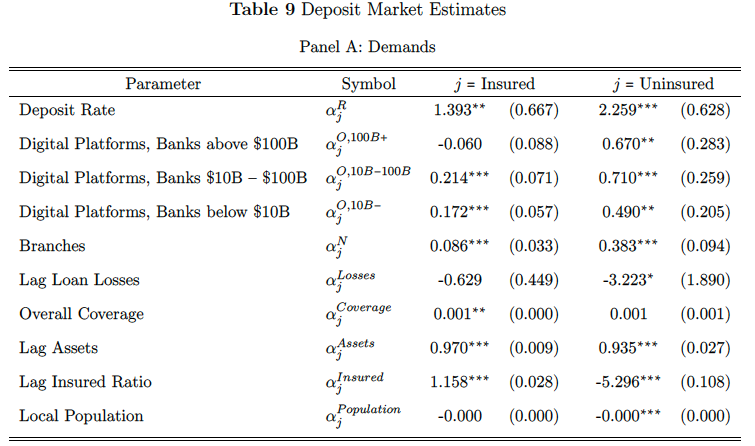
\includegraphics[width=0.8\textwidth]{imgs/tab9.png}
        %\caption*{Caption}
        % \label{fig:my_label}
    \end{figure}
    
    \end{frame}

    \begin{frame}{Deposits Cost estimation results}\label{cost_results}


        \begin{figure}
            \centering
            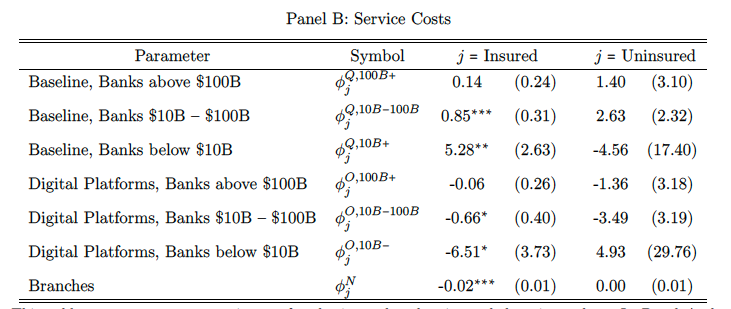
\includegraphics[width=0.8\textwidth]{imgs/tab9b.png}
            %\caption*{Caption}
            % \label{fig:my_label}
        \end{figure}
        
        \end{frame}
    
        \begin{frame}{Demand and cost for loans results}\label{demand_cost_loans}


            \begin{figure}
                \centering
                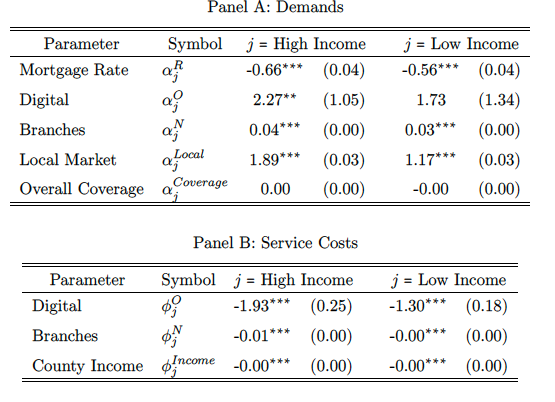
\includegraphics[width=0.6\textwidth]{imgs/tab10.png}
                %\caption*{Caption}
                % \label{fig:my_label}
            \end{figure}
            
            \end{frame}


        \begin{frame}{Loan losses estimation results}\label{loan_losses}

            \begin{figure}
                \centering
                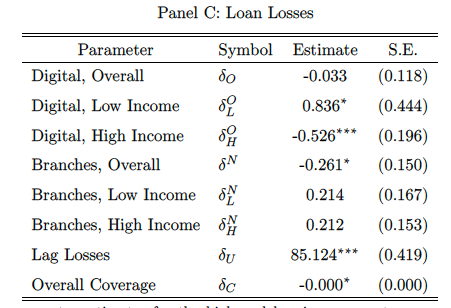
\includegraphics[width=0.5\textwidth]{imgs/tab10c.png}
                %\caption*{Caption}
                % \label{fig:my_label}
            \end{figure}
            
            \end{frame}

            \begin{frame}{Banks fixed costs estimation results}\label{fixed_costs}

                \begin{itemize}
                    \item Bounds for fixed costs are:
                    \item E.g. entry cost between mile distance to headquarter range from 10\$ to 318\$.
                \end{itemize}

                \begin{figure}
                    \centering
                    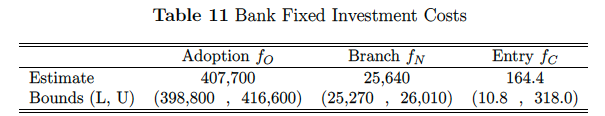
\includegraphics[width=0.6\textwidth]{imgs/tab11.png}
                    %\caption*{Caption}
                    % \label{fig:my_label}
                \end{figure}
                
            \end{frame}

            \begin{frame}{Aggregate Effects on Competition}\label{agg_effects}
                \begin{itemize}
                    \item Concentration decreases with digital platforms.
                \end{itemize}



                \begin{figure}
                    \centering
                    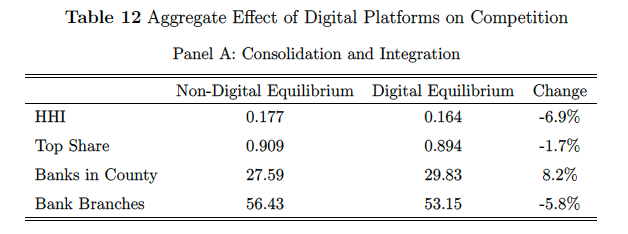
\includegraphics[width=0.6\textwidth]{imgs/tab12.png}
                    %\caption*{Caption}
                    % \label{fig:my_label}
                \end{figure}
                
            \end{frame}

            \begin{frame}{Competition Implications}\label{comp_implications}   

                % \begin{itemize}
                %     \item Concentration decreases with digital platforms.
                % \end{itemize}

                \begin{figure}
                    \centering
                    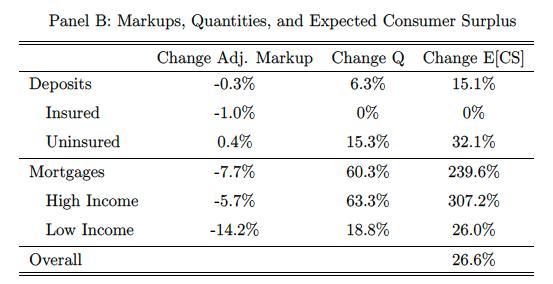
\includegraphics[width=0.6\textwidth]{imgs/tab12b.png}
                    %\caption*{Caption}
                    % \label{fig:my_label}
                \end{figure}
                
                \begin{figure}
                    \centering
                    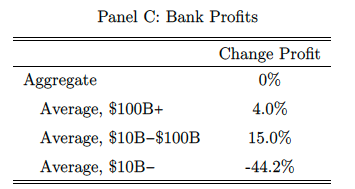
\includegraphics[width=0.34\textwidth]{imgs/tab12c.png}
                    %\caption*{Caption}
                    % \label{fig:my_label}
                \end{figure}
            \end{frame}




            \begin{frame}{Financial Stability implications}\label{fin_stab}

 Midsize banks provide more services and serve more markets. Avg. expected loan losses decrease.
                \begin{figure}
                    \centering
                    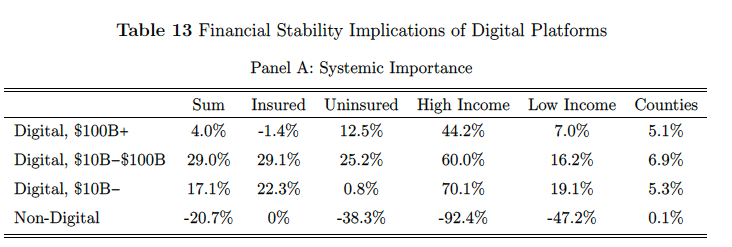
\includegraphics[width=0.6\textwidth]{imgs/tab13.png}
                    %\caption*{Caption}
                    % \label{fig:my_label}
                \end{figure}
                
                \begin{figure}
                    \centering
                    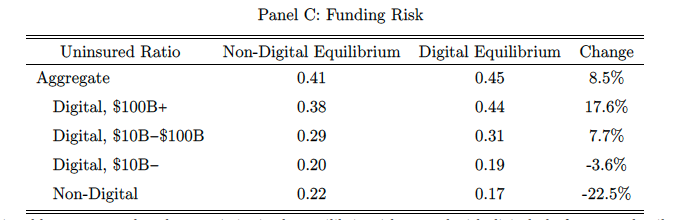
\includegraphics[width=0.55\textwidth]{imgs/tab13c.png}
                    %\caption*{Caption}
                    % \label{fig:my_label}
                \end{figure}
            \end{frame}

     






% Conclusion frame

\begin{frame}{Conclusion}
    % \begin{wideitemize}
        % \item \textcolor{blue}{Summary:} 
        \begin{wideitemize}

            \item Documents Digital platforms increase competition and pose risks to financial stability. 
            \item Midsize banks benefit from the adoption of digital platforms.
            \item Likely to have implications for monetary policy and financial regulation.
        \end{wideitemize}

    \end{frame}
    

    \begin{frame}{}
        % Thank you slide
        \centering
        \huge \textcolor{blue}{Thank you!}
    \end{frame}


    


\end{document}